\chapter{Experiments and results}

\section{Datasets}

Several datasets were examined, and the most suitable was selected for our task. Large portion of datasets for 3D reconstruction contain depth maps, key points, but not RGB image: NYU, ICVL, MSRA15, BigHand2.2M, SynHand5M, FHAD, MSRC\(FingerPaint\), HandNet, Hands in Action, MSRA14 \cite{1,2,3,4,15,16,17,18,19,20}. For the problem of reconstruction from a single image, most appropriate datasets are those that feature both RGB records and key points: FreiHAND, GANerated Hands, EgoDexter, SynthHands, STB, Dexter+Object, UCI-EGO, MHP \cite{4, 11, 12, 14, 21, 22}. The possible complication of combining different datasets is that the number of key points, record types, and camera parameters may not match. We left only datasets with a central position of a hand and 21 labeled key points.

FreiHAND Dataset is a hand pose dataset for hand pose estimation from a single image. The dataset contains shots with 4 different data augmentations annotated with 21 key points for 2D and 3D spaces. The total amount of training samples is 130240 for single view training. So 32560 poses for training \cite{4}. 

GANerated Hands Dataset contains 330,000 examples annotated with 21 key points for 2D and 3D spaces. The downside of this dataset is that images are synthetically generated and have distorted edges of hands. All of them are recorded from one viewpoint \cite{11}.

SynthHands is a synthetic dataset, which provides information about 63,530 frames recorded from 5 views. Learning examples contain both RGB and depth records and represent records with and without object interaction. Data annotated for 21 points in 3D space. Hands were generated using Unity3D engine but animated using data captured from real motion \cite{12}. 

We chose FreiHAND Dataset and SynthHands dataset for training and evaluation, respectively. Also, we used Home Object Dataset for background augmentation of SynthHands dataset. Home Object Dataset \cite{HOD} contains 450 photos of random objects. Augmented SynthHand dataset denoted in work as 'SynthHands\_A'.

\begin{table}
\begin{tabularx}{1\textwidth} { 
  | >{\raggedright\arraybackslash}X 
  | >{\centering\arraybackslash}X 
  | >{\centering\arraybackslash}X 
  | >{\raggedleft\arraybackslash}X | }
 \hline
 Dataset name & Number of images & Synthetic / Real  & Number of camera views \\
 \hline
 FreiHAND  & 32,560  & Real  & 1 \\
 \hline
 GANerated Hands  & 330,000  & Synthetic  & 1 \\
 \hline
 SynthHands  & 63,530  & Synthetic  & 5 \\
\hline
\end{tabularx}
\caption{\label{tab:table-name}Datasets info}
\end{table}

Besides annotated datasets for training and testing, we used the ASL dataset for reconstructions. Kaggle ASL dataset \cite{ASL} contains 87000 of hand poses. Images were labeled for the task of sign language recognition. There are 26 classes for letters and three classes with images for SPACE, DELETE, and NOTHING.

\section{Data preprocessing algorithms}

As there were no 3D annotated video dictionaries of sign language available at the time of the study, an artificial sequencing procedure was proposed. It is proposed to sort images of hands with annotations to mimic real-world transition of hands from frame to frame. For each record in a dataset, we search one with the closest 3D position and use both in the training process. Because frame n and n-1 have close 3D positions in the real world, such sorting allows us to use a non-video dataset for usage in tasks of video processing. Usage of fake video sequences different from real-world applications in two ways. First - the transition between hands not as smooth as in the real world. Second - in our study, we used ground truth annotation for the previous frame at the input for the network. Because the previous frame is more random than in real videos - ground truth data in a way mimic noisy prediction for the previous frame. But, of course, training on annotated synthetic video does not suffer from an accumulation of noise as much as if for each next frame, we would use the previous prediction of the network.

To solve the task of shape reconstruction, we are adding additional data preprocessing. First, we are masking density estimation of MANO annotations to sample more data. We are creating a new dataset by sampling vectors from distribution, passing it to a MANO model, and obtain corresponding 3D shape and key-points. The new dataset allows us to train network C on a large number of sampled vectors. 

\section{Training 3D shape estimation stages}

For training and testing was used Frei Hand Dataset split for test and train subsets in ratio 1:4. As an additional dataset for evaluation, we used SynthHand dataset with and without the addition of background.

It is needed to account for different scales of key point spaces. Datasets or hand models encode certain magnitude of hand, so simultaneous work with different coordinates requires unification. In our case MANO model, Synth Hand Dataset and Frei Hand Dataset are all in different scales. Frei Hand Dataset hands are ~990 times smaller than MANO reconstructions. In contrast, Synth Hand Dataset is ~0.94 times smaller than MANO hands. It does not influence training for 2D key-points because data projected to the image plane and unified in that way. For depth, it is more important to have annotation in one scale. Networks for depth estimation learn both ratios between fingers depth as well as absolute depth. We have transformed the absolute depth of SynthHand Dataset annotations to match the average depth of FreiHand Dataset. For calculation of 3D error, we transformed all coordinates to MANO model space. It is the shortest way to achieve unification given that vector of MANO parameters is part of our pipeline, and that scale is used for training.

% ###################################################################################################################################
\subsection{Training and testing of networks for 2D key-point detection} 

We trained and tested 6 architectures in parallel. Adam optimizer was used with learning rate 0.0001 and trained on mini-batches of size 4 from FreiHand dataset for 40820 steps. We tested Mean Squared Error of predicted probabilities of location for each key point as well as absolute distance between the predicted location of key point and ground truth in 2D. For each network, we tested performance on 300 random images from 4 datasets. Results of testing on the train and test subsets of FreiHand Dataset are presented in tables 4.4 and 4.5, respectively. Metrics measured on Synth Hand Dataset presented in Table 4.6 for data without background, and table 4.7 tests on images with augmented backgrounds.

Results in tables 4.2-4.5 show that providing additional video frames decreases mean errors in most cases by 5-30\%. And additional refinement improves results only after a certain number of iteration. The proposed variation of Stack Hourglass Model has better results than larger UNET architecture on train subset as well on Synth Hand data-set with and without background. But since it has a larger error on test subset on real data, we assume that UNET generalizes better.

\begin{table}[H]
\small
\begin{tabularx}{1\textwidth}{sbbbbbb}
 \hline
 & STH\_2\_PIC & STH\_2\_VID & STH\_3\_PIC & STH\_3\_VID & UNET\_PIC & UNET\_VID \\
 \hline
mse \\
(points) &
2.64E+02 &
1.63E+02 &
1.92E+02 &
1.67E+02 &
2.15E+02 &
1.16E+02 
\\
\hline
l1 \\
(points)&
10.097 &
7.198 &
7.861 &
7.545 &
7.192 &
6.259 
\\
\hline
mse \\
(heatmaps) &
8.11E-04 &
7.68E-04 &
7.89E-04 &
7.82E-04 &
7.60E-04 &
7.62E-04 
\\
\hline
\end{tabularx}
\caption{\label{tab:res_1}Mean errors on train dataset for networks A}
\end{table}

\begin{table}[H]
\small
\begin{tabularx}{1\textwidth}{sbbbbbb}
 \hline
 & STH\_2\_PIC & STH\_2\_VID & STH\_3\_PIC & STH\_3\_VID & UNET\_PIC & UNET\_VID \\
 \hline
mse \\
(points)&
2.86E+02 &
2.01E+02 &
2.17E+02 &
1.89E+02 &
1.92E+02 &
1.67E+02 
\\
\hline
l1 \\
(points)&
10.582 &
8.448 &
8.507 &
8.59 &
6.906 &
7.757 
\\
\hline
mse \\
(heatmaps) &
8.26E-04 &
8.11E-04 &
8.09E-04 &
8.24E-04 &
7.77E-04 &
7.99E-04 
\\
\hline
\end{tabularx}
\caption{\label{tab:res_2}Mean errors on test dataset for networks A}
\end{table}

\begin{table}[H]
\small
\begin{tabularx}{1\textwidth}{sbbbbbb}
 \hline
 & STH\_2\_PIC & STH\_2\_VID & STH\_3\_PIC & STH\_3\_VID & UNET\_PIC & UNET\_VID \\
 \hline
mse \\
(points)&
8.66E+02 &
6.62E+02 &
7.47E+02 &
3.66E+02 &
8.91E+02 &
4.02E+02 
\\
\hline
l1 \\
(points)&
20.327 &
15.222 &
18.373 &
11.857 &
21.03 &
12.5 
\\
\hline
mse \\
(heatmaps) &
8.87E-04 &
8.47E-04 &
8.86E-04 &
8.33E-04 &
9.15E-04 &
8.42E-04 
\\
\hline
\end{tabularx}
\caption{\label{tab:res_3}Mean errors on SynthHand dataset for networks A}
\end{table}


\begin{table}[H]
\small
\begin{tabularx}{1\textwidth}{sbbbbbb}
 \hline
 & STH\_2\_PIC & STH\_2\_VID & STH\_3\_PIC & STH\_3\_VID & UNET\_PIC & UNET\_VID \\
 \hline
mse \\
(points)&
8.61E+02 &
5.34E+02 &
8.33E+02 &
5.41E+02 &
1.15E+03 &
4.24E+02 
\\
\hline
l1 \\
(points)&
21.201 &
14.359 &
20.305 &
14.486 &
24.221 &
13.042 
\\
\hline
mse \\
(heatmaps) &
9.04E-04 &
8.69E-04 &
9.12E-04 &
8.76E-04 &
9.13E-04 &
8.68E-04 
\\
\hline
\end{tabularx}
\caption{\label{tab:res_4}Mean errors on SynthHand\_A dataset for networks A}
\end{table}

% ###################################################################################################################################
\subsection{Training and testing of networks for Depth detection}

We trained and tested in parallel 4 architectures, their id's start with B. We have used Adam optimizer with learning rate 0.01 and trained on mini-batches of size 64 from FreiHand dataset for 5719 steps. We trained networks to predicted relative distances between fingers as well as the tilt of the hand as the 22nd parameter. We measured the absolute distance between predicted and ground-truth values of depth for each key point. Also, we measured errors of predictions for relative positions of fingers and hand tilt. 

Network AB\_PIC was trained for the labeling of sing language letters. We pretrained UNET architecture for ~141800 steps with batch size 16 and used Adam optimizer with a learning rate 0.001. We have used U-Net as a basis on top of which trained depth estimator for ~44000 steps with batch size 8 and used Adam optimizer with learning rate 0.001.

Measurement on splitted FreiHand dataset shown in table 4.6 for training data, 4.7 for test data. Tables 4.8 and 4.9 present values of metrics on Synth Hand Dataset for default and augmented data, respectively. 

From tables we can see that the usage of additional frames improves the quality of depth estimation. Additional refinement improves quality for all cases except synthetic data without data augmentation. AB\_PIC has the best results among architectures for single image analysis. 

\begin{table}[H]
\small
\begin{tabularx}{1\textwidth}{sbbbbb}
 \hline
 & B0\_VID &
   B0\_PIC &
   B1\_VID &
   B1\_PIC &
   \textbf{AB\_PIC} \\
 \hline
    mse \\
(network \\
output)&
1.13E-02 &
1.83E-02 &
1.69E-02 &
1.91E-02 &
\textbf{1.07E-02} 
\\
\hline
l\_1 \\
(network \\
output)&
7.29E-02 &
9.57E-02 &
9.22E-02 &
9.97E-02 &
\textbf{7.70E-02} 
\\
\hline
\hline
l\_1 \\
(depth)&
1.21E-02 &
1.40E-02 &
1.45E-02 &
1.54E-02 &
\textbf{1.04E-02} 
\\
\hline
\end{tabularx}
\caption{\label{tab:res_5}Mean errors for networks B on train dataset}
\end{table}


\begin{table}[H]
\small
\begin{tabularx}{1\textwidth}{sbbbbb}
 \hline
 & B0\_VID &
   B0\_PIC &
   B1\_VID &
   B1\_PIC &
   \textbf{AB\_PIC} \\
 \hline
 mse \\
(network \\
output) &
1.75E-02 &
2.19E-02 &
2.76E-02 &
2.08E-02 &
\textbf{1.49E-02}
\\
\hline
l\_1 \\
(network \\
output) &
9.12E-02 &
1.01E-01 &
1.15E-01 &
1.06E-01 &
\textbf{8.92E-02}
\\
\hline
\hline
l\_1 \\
(depth) &
1.33E-02 &
1.55E-02 &
1.69E-02 &
1.52E-02 &
\textbf{1.15E-02}
\\
\hline
\end{tabularx}

\caption{\label{tab:res_6}Mean errors for networks B on test dataset}
\end{table}


\begin{table}[H]
\small
\begin{tabularx}{1\textwidth}{sbbbbb}
 \hline
 & B0\_VID &
   B0\_PIC &
   B1\_VID &
   B1\_PIC &
   \textbf{AB\_PIC} \\
 \hline
 mse \\
(network \\
output) &
2.92E-02 &
1.90E-01 &
1.87E-02 &
1.81E-01 &
\textbf{8.63E-02}
\\
\hline
l\_1 \\
(network \\
output) &
1.31E-01 &
3.51E-01 &
1.01E-01 &
3.54E-01 &
\textbf{2.47E-01}
\\
\hline
\hline
l\_1 \\
(depth) &
2.05E-02 &
7.14E-02 &
1.61E-02 &
4.10E-02 &
\textbf{2.79E-02}
\\
\hline
\end{tabularx}

\caption{\label{tab:res_7}Mean errors for networks B on SynthHand dataset}
\end{table}

\begin{table}[H]
\small
\begin{tabularx}{1\textwidth}{sbbbbb}
 \hline
 & B0\_VID &
   B0\_PIC &
   B1\_VID &
   B1\_PIC &
   \textbf{AB\_PIC} \\
 \hline
mse \\
(network \\
output)&
2.45E-02 &
2.01E-01 &
2.54E-02 &
1.63E-01 &
\textbf{8.10E-02}
\\
\hline
l\_1 \\
(network \\
output) &
1.18E-01 &
3.65E-01 &
1.17E-01 &
3.25E-01 &
\textbf{2.24E-01}
\\
\hline
\hline
l\_1 \\
(depth) &
1.79E-02 &
4.32E-02 &
2.07E-02 &
3.83E-02 &
\textbf{2.79E-02}
\\
\hline
\end{tabularx}
\caption{\label{tab:res_8}Mean errors for networks B on SynthHand\_A dataset}
\end{table}

% ###################################################################################################################################
\subsection{Training and testing of networks for shape parameterisation}

At first we tested multilayer perceptrons with various architectures and various losses, but results always were unsatisfying and could be generalized to two scenarios. The first one is the total inability of the network to learn hand 3D parametrization, and second is remembering of avg hand. We tested dropout and normalization layers, loss of parameters only, loss of both parameters, and hand shape reconstruction. In the end, we have selected the best performing of our perceptrons and compared its performance with the LSTM network.

'C\_MLP' was trained for 1183 steps. Training setting: Adam optimizer, learning rate = 0.01, batch size = 16384. LSTM was trained for 2400 steps with the same learning rate, but batch size 2048.

Results of how well networks preserve the position of 3D key-points after decoding of estimated parameters are shown in Table 4.10. 'C\_RNN' network turned out to be more precise in performed tests.

\begin{table}[H]
\small
\begin{tabularx}{1\textwidth}{sbb}
 \hline
 & RNN &
   MLP \\
 \hline
mse &
145.25008 &
286.72867 
\\
\hline
l\_1 &
5.887265 &
9.51802 
\\
\hline
\end{tabularx}
\caption{\label{tab:res_9}Mean errors for C networks}
\end{table}

% ###################################################################################################################################
\section{Annotation system analysis}

We have combined AB\_PIC network with proposed RNN for shape parameterization and tested how the addition of shape influences predicted positions of key points. The results of the experiments are shown in Table 4.11.

\begin{table}[H]
\small
\begin{tabularx}{1\textwidth}{bbbbb}
 \hline
 & TRAIN &
   TEST &
   SynthHands &
   SynthHands\_A \\
 \hline
 \hline
MSE AB\_PIC &
267.01346 &
329.91776 &
2865.1726 &
3540.065 

 \\
\hline
l1 AB\_PIC &
11.493821 &
12.303339 &
39.867397 &
44.1231 

\\
\hline
\hline
MSE MANO &
322.8869 &
360.14267 &
3814.0867 &
4494.155 

\\
\hline
l1 MANO &
12.073699 &
12.662715 &
46.253853 &
50.823338 
\\
\hline
\hline
Deviation &
4.8\% &
2.9\% &
13.8\% &
13.2\%
\\
\hline
\end{tabularx}
\caption{\label{tab:res_10}Intermediate and final 3D key point errors}
\end{table}

First two rows inform how far predicted points deviate from the ground truth. We see the same pattern of descending accuracy for unseen data as in tables from 4.2 to 4.9. Rows 3,4 show the accuracy of key-points extracted from the MANO 3D model (Fig 3.3 a)). 
The final row reflects the impact of adding hand surface on key points position.

From tables from 4.2 to 4.11 we see that error on SynthHands Dataset always significantly larger. Fig 4.1 to 4.3 show images presented in 3 datasets. On top, we see detected 2D key points and at the bottom predicted 3D shapes. 3D shapes displayed reflected and rotated due to the camera position of rendering software. Predicted shape and points are actually not rotated that way and transformed only by scaling and translation.

\begin{figure}[H]
\caption{Examples of FreiHand 3D reconstructions}
\centering
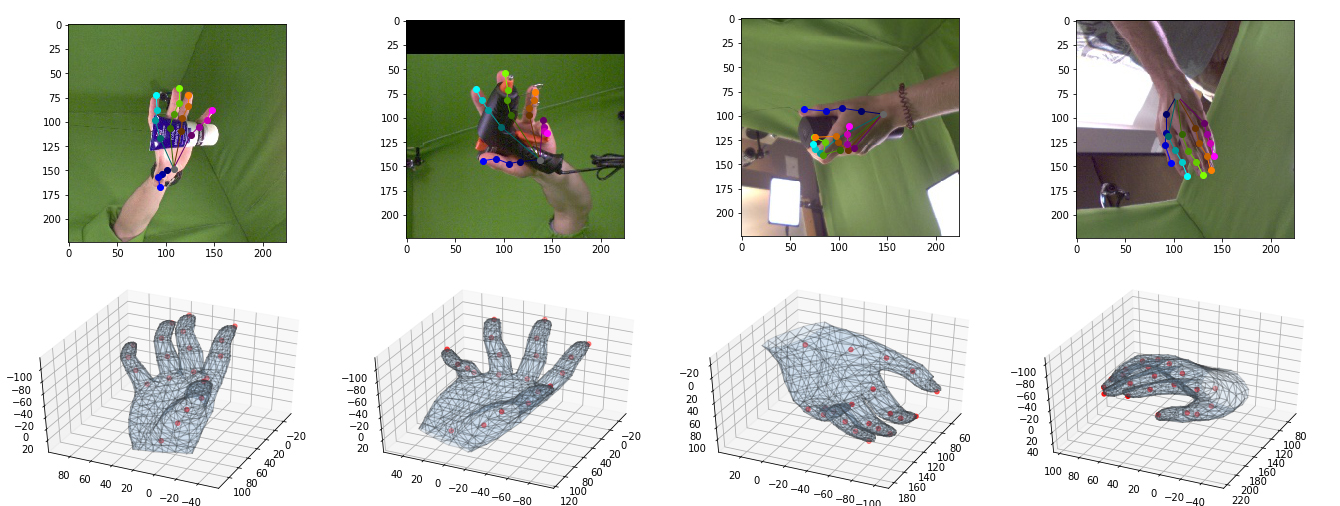
\includegraphics[width=1\textwidth]{fh}
\end{figure}

On Fig 4.1 we see accurate detection of key-point on Frei Hand Dataset. Even occluded points predicted on 2D and 3D. For instance, 3rd image from the left at Fig 4.1 show the accurate prediction of occluded little finger, which is seen at reflected reconstruction at the bottom.

\begin{figure}[H]
\caption{Examples of SynthHands\_A 3D reconstruction}
\centering
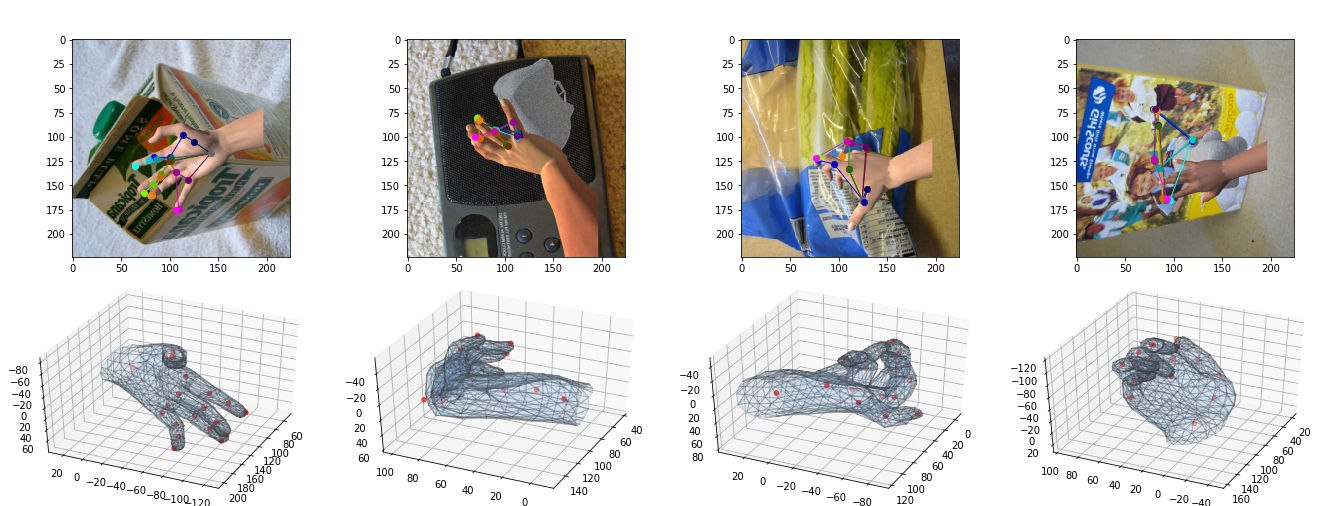
\includegraphics[width=1\textwidth]{sh_expls}
\end{figure}

In Fig 4.2 we see images from Synth Hand Dataset with an augmented background. The errors obtained on the SynthHands\_A dataset was the largest among all tests. Top images show a misdetection of 2D points. Now we can better understand a larger deviation of 3D model from 3D key-points detected by network AB\_PIC. Network C\_RNN estimates MANO parameters that encode some anatomy by design. The final shape it creates is more realistic than detected 3D points by AB\_PIC. 

\begin{figure}[H]
\caption{Examples of ASL 3D reconstruction}
\centering
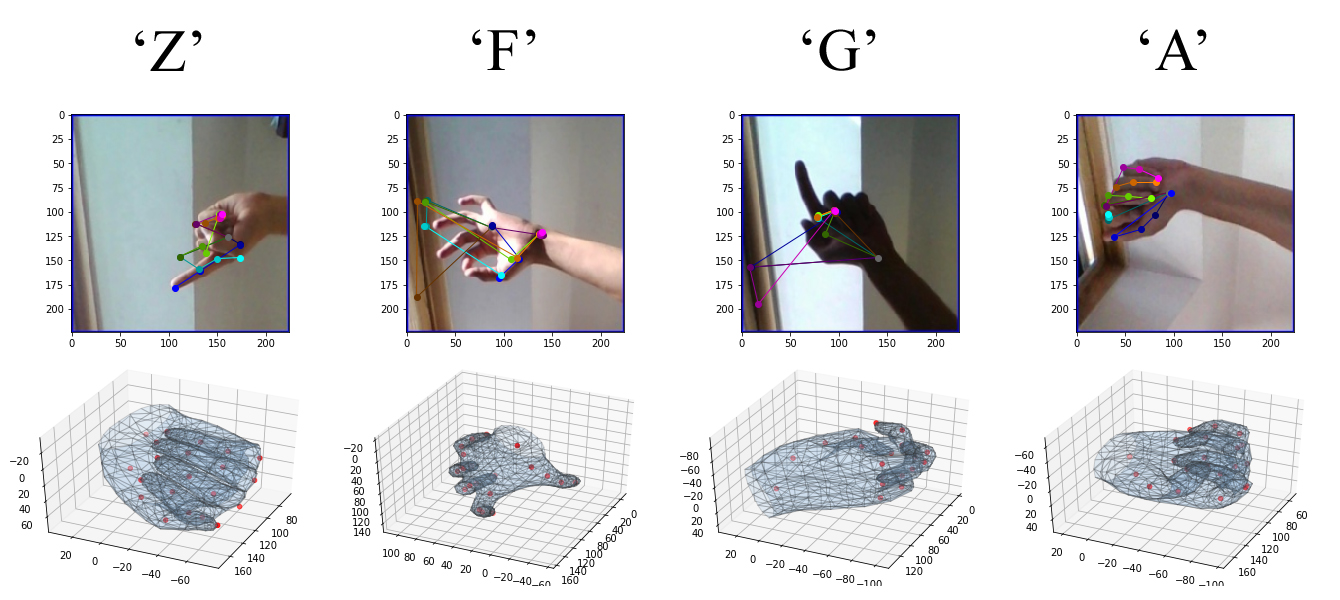
\includegraphics[width=1\textwidth]{alphabet}
\end{figure}

On Fig 4.3 we see predicted hand shapes for ASL. Most shapes mismatch originals. Even though in some cases, as for letter 'A' we see that the system can accurately reconstruct sign language pose. It is also a good example of how the final shape can fix misdetected points. 2D Key Points and depth were undetected on an index finger, but the final shape filled them to match the anatomy of the hand.